\documentclass[a4paper, 11pt]{article}
\usepackage[a4paper, margin=3cm]{geometry}
\onecolumn
\usepackage[english]{babel}

\usepackage{graphicx}
\usepackage{amsmath, amssymb, amsthm}
\usepackage{xcolor}
\usepackage{listings}
\usepackage{etoolbox}
\usepackage{caption}
\usepackage{cleveref}

\makeatletter
\AtEndEnvironment{lstlisting}{\xdef\xlang{\lst@language}}
\AfterEndEnvironment{lstlisting}{
  \vspace*{-1.5em}
  \begin{flushright}\xlang
\end{flushright}}
\makeatother

\lstdefinelanguage{Logo}{
  morekeywords={to, end, forward, back, clearscreen, penup, pendown, print, fd, backward, bk, right, rt, left, lt, repeat, stop, sqrt, if, ifelse, while, for},
  sensitive=false,
  morecomment=[l]{;},
  alsoletter={:},
  moredelim=[s][\color{orange}]{:}{\ }
}

\lstset{
  language=Logo,
  basicstyle=\ttfamily\small,
  keywordstyle=\color{blue}\bfseries,
  commentstyle=\color{green!60!black},
  numbers=left,
  numberstyle=\tiny\color{gray},
  frame=single,
  breaklines=true
}

\usepackage{csquotes}
\usepackage[backend=biber, style=numeric]{biblatex}
\addbibresource{literatur.bib}

\title{Recursion, Fractals and space-filling curves in Logo}
\author{Alina Musaeva \and Julian Schwarzer \and Lars Wittner}
\date{June 2026}

\begin{document}

\maketitle

\section*{Abstract}
This paper introduces Logo as a functional programming language, focusing on recursion as the basis for fractals. These are key concepts for grasping how Logo can be utilised to generate space-filling curves. We will also explain L-systems and the fundamental mathematics behind them. We will go through the base commands and view a few examples of recursion, as well as explaining how to create fractals in different ways. Topics covered will include edge- and node-rewriting.

\section{Introduction}

In chapter \Cref{sec:definitionlog} we will explore what Logo is, its main features and how to work with it. We will show you some base commands which are required to better understand it in other chapters. In chapter \Cref{sec:recursion} and \Cref{sec:fractals} , we will methodically explore the concepts of recursion and fractals using the Pythagoras tree, Koch's flake. Finally, we will cover topics such as L-system, edge- and node-rewriting and branching in chapter \Cref{sec:Lsystem}. This will enable you to understand the idea of space-filling curves in Logo.

\section{Definition of Logo and its origin}
\label{sec:definitionlog}
Before we move on to recursion and fractals, we're going to find out what Logo is and learn some base commands.

Logo is a programming language that is well-known for its use of turtle graphics. With Logo, you can draw different figure shapes.

It was invented in 1966 in Cambridge (USA) by Wally Feurzeug, Seymour Papert, Daniel Bobrow and Cynthia Solomon.

The original intention behind the creation of this language was to provide a means for children in schools to learn how to code and enhance their mathematical skills \cite{history}.

\subsection{Turtle Graphics}
\label{sec:turtleg}
The turtle is a pen or a cursor (often represented as a triangle) that moves after a command and draws when the pen is down. You can change the position, direction, pen state, color etc. It will all be displayed on the computer screen \cite{lieberman}.

\subsection{Data Types}
\label{sec:datatypes}
In Logo, data types are dynamic. This means that they do not need to be defined explicitly.

There are four main data types: word, number, list and boolean \cite{datatypes}.

\begin{enumerate}
  \item \textit{word} is used for a sequence of characters
  \item \textit{number} for such numbers as integer, float, double etc.
  \item \textit{list}  is a list of numbers or characters (which may for example be a sentence or an array).
  \item \textit{bool} is for true or false
\end{enumerate}

\subsection{Base commands}
\label{sec:basecommands}
The Logo syntax is very intuitive. It consists of simple words, with or without parameters (\Cref{fig:abb1}).

A shortcut is also available for each command, thus avoiding the need to type the entire word each time.

Here are the base commands \cite{procedures}:

\begin{verbatim}
FORWARD/BACK steps
RIGHT/LEFT degree
CLEARSCREEN
PENUP/PENDOWN
REPEAT
PRINT [The sentence]
\end{verbatim}

As demonstrated in \Cref{fig:abb1}, the turtle was moved forward 40 steps, rotated 110 degrees, and moved forward again 49 steps.

\begin{figure}[h]
  \centering
  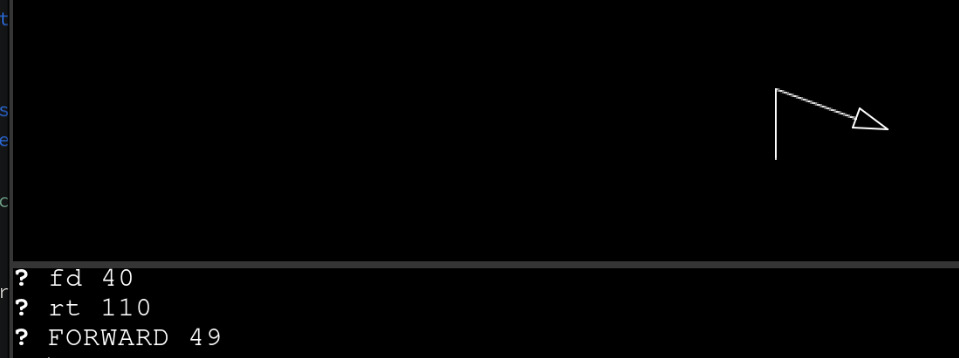
\includegraphics[width=10cm]{images/bc1.jpeg}
  \caption{command forward and right in ucbLogo}
  \label{fig:abb1}
\end{figure}

The others commands for instance \texttt{CLEARSCREEN} or simply \texttt{CS} is used for cleaning the drawings on the display (not the code).

\texttt{PENUP} is used to move the turtles position without drawing and \texttt{PENDOWN} to return to the drawing mode.

\texttt{REPEAT} allows commands to be repeated multiple times, thus saving time.

For example we can draw a square using following command:

\begin{lstlisting}
REPEAT 4 [fd 90 rt 90]
\end{lstlisting}

To print words, numbers or lists we use the following syntax in logo:
\begin{lstlisting}[caption=Examples of printing]
Print "word
Print 8
Print [Hello world]
Print [1 2 4]
\end{lstlisting}

\begin{lstlisting}[caption=Output of Listing 1]
 word
 8
 Hello world
 1 2 4
\end{lstlisting}

\subsection{Procedures}
The following steps are required to create a procedure (function) in Logo:

Enter \textit{To} followed by the name of the procedure and \textit{End}. The commands should then be entered between these two items. Use parameters if required.

\begin{lstlisting}
To ProcedureName :parameter1 ... :parameterN
    commands
End
\end{lstlisting}

For example, we can now create a procedure that enables us to draw different polygons.

\begin{lstlisting}
To PolygonMaker :num1 :len
    repeat :num1 [ fd :len rt 360/:num1]
End
\end{lstlisting}

\begin{figure}[h]
  \centering
  \fbox{
    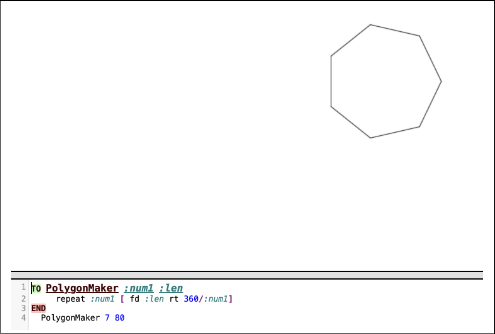
\includegraphics[width=10cm]{images/pol.png}
  }

  \caption{Call of procedure PolygonMaker}
  \label{fig:polygon}
\end{figure}

In this procedure we used 2 parameters \textit{num1} - number of angles and  \textit{len} - length of the sides. So now we can use it to make a triangle, a square, an octagon or even a circle. Besides, this function can be called multiple times.

\subsection{Loops}
Also a very important part of almost every programming language are loops and if else statement.

\begin{lstlisting}[title=If/Ifelse statement]
IFELSE condition [condition true][condition false]
IF condition [condition true]
\end{lstlisting}

Logo is very intuitive. We enter  \textit{ifelse}  and a condition that will be proven to be either true or false. The corresponding command will then be called.
Or simply use \textit{if} if you only have one if-case \cite{datatypes}.

\begin{lstlisting}[title=While-loop]
WHILE [condition]
[commands]
\end{lstlisting}

The while loop is also pretty simple. First, we enter \textit{While}, then the condition. After that, we enter the commands that will be executed while the statement is true.

\begin{lstlisting}[title=For-loop]
FOR [var start end step]
[commands]
\end{lstlisting}

The For loop is slightly different to that in other programming languages. First, we type \textit{For} and then four parameters in braces: the name of the variable, the starting value, the ending value, and the step value. After this, we can enter commands that will be executed within the loop.

\begin{lstlisting}[caption=Example of using For loop]
for [i 1 10 2]
[print :i]
\end{lstlisting}

\begin{lstlisting}[caption=Output of Listing 3]
1
3
5
7
9
\end{lstlisting}

\section{Recursion}
\label{sec:recursion}
We are now capable of writing programs with these base commands but we still have to introduce recursion for a functional programming language like Logo.

\subsection{Definition}
Recursion has its origin in the latin word \textit{recurrere (to go back)}. A recursive written function has to contain three key parts:

\begin{enumerate}
  \item Base case
  \item Calling itself
  \item Recursive step
\end{enumerate}

The base case will be a condition that indicates what case our recursive calls will end up terminating.
We need this due to our limitations of storage and to avoid an infinite number of calls on our call stack.
To actually reach this base case we need a recursive step that needs to be provided by our recursive call that approaches our base case \cite{geeksforgeeks}.

\begin{lstlisting}[title={Fibonacci numbers}, language=Java, label={lst:fibonacci}]
  private static int fib(int n) {
    if (n <= 0) return -1; // wrong input
    if (n == 1) return 0; // base case 1
    if (n == 2) return 1; // base case 2
    return fib(n - 1) + fib(n - 2); // recursive call
  }
\end{lstlisting}

In this java implementation of the Fibonacci numbers (\Cref{lst:fibonacci}) you can see that there are also multiple base cases possible.
For this example the first Fibonacci number is defined to be "0" and the second one has to be "1". After these base cases the recursive call and its embedded recursive steps will give us our final result of our requested $n$th number.
As you might have noticed the recursive step is not only one time but two times in this example. This is because the Fibonacci numbers are defined as the sum of the previous two numbers.

It is very important that the recursive step actually reaches our base case. In this example each reduction (\(n-1\) and \(n-2\)) will either reach our first or our second base case and terminate.
If we had skipped our base case and had not filtered wrong inputs by \(n<=0\) the method would not terminate and the recursion will end up in an infinite loop.

The phrase \textit{depth of recursion} determines the amount of nested recursive functions inside of itself.

Recursion often finds usage in science like mathematics \textit{eg. factorials, Fibonacci} or computer science like in functional programming languages like Logo that profit from reduced lines of code and readability.

\subsection{ Pythagoras tree}

\begin{figure}[t]
  \centering
  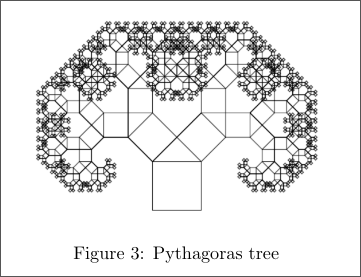
\includegraphics[width=0.5\textwidth]{images/pythagoras_tree.png}
  \caption{Pythagoras tree}
  \label{fig:Pythagoras tree}
\end{figure}

The pythagoras tree is a very common example to explain recursion \cite{mathworld}.
Its main shape is a square with recursively placed squares on top of the base square rotated by a predefined angle that is calculated based on the famous Pythagoras formula (\Cref{fig:Pythagoras tree}).

To implement this, we will use the previously explained scheme: We declare our procedure within the first line (keyword \textit{to}) with its name being \textit{pythagoras} and two needed parameters (indicated by the colons) as \textit{length} and \textit{depth}. We end our definition with the keyword \textit{end} in our last line.

\begin{lstlisting}
  to pythagoras :length :depth
    ...
  end
\end{lstlisting}

First, we implement our main shape (the square) by repeating it four times going forward and turning right.

\begin{lstlisting}
  repeat 4 [fd :length rt 90]
\end{lstlisting}

Now we write our base case, which means terminating our program at depth=0. The depth represents the maximum number of squares placed on top of each other (\textit{recursion depth}).

\begin{lstlisting}
  if :depth = 0 [stop]
\end{lstlisting}

We end up at our starting position at the left bottom corner of the just drawn square. To draw our recursive squares, we need to correct our position.

For that we have to reach the top left corner and rotating to the left by 45 degree, which will be our predefined rotation, so both squares will have the exact same length and our Pythagoras tree becomes axially symmetric.

\begin{lstlisting}
  fd :length lt 45
\end{lstlisting}

Our recursive squares are then drawn with a reduced length in the scale of the Pythagoras formula and a depth that decreases by "1", which ensures the base case of depth=0 being reached at some point.

\begin{lstlisting}
  pythagoras :length / (sqrt 2) :depth - 1
\end{lstlisting}

Because we are using the 45 degree angle, the following derivation explains the new length:
We assume our hypotenuse as \textit{a} and our two catheti as length \textit{b}.

According to Pythagoras:

\begin{align*}
  a^2 + a^2 &= b^2 \\
  2a^2 &= b^2 \\
  \sqrt{2}a &= b \\
  b &= \frac{a}{\sqrt{2}}
\end{align*}

We have to change our position again to start the second recursive square.

\begin{lstlisting}
  rt 90 fd :length / (sqrt 2)
\end{lstlisting}

Positioned correctly, we perform the same recursive call as our first part.

\begin{lstlisting}
  pythagoras :length / (sqrt 2) :depth - 1
\end{lstlisting}

After each recursive depth, we return to the position of the previous one (\textit{depth + 1}).

\begin{lstlisting}
  bk :length / (sqrt 2) lt 45 bk :length
\end{lstlisting}

The result of our final procedure will be as follows:

\begin{lstlisting}[title={Pythagoras tree}]
to pythagoras :length :depth ; variable length and depth
  repeat 4 [fd :length rt 90] ; square
  if :depth = 0 [stop] ; base case
  fd :length lt 45 ; change pos
  pythagoras :length / (sqrt 2) :depth - 1 ; recursive left
  rt 90 fd :length / (sqrt 2) ; change pos
  pythagoras :length / (sqrt 2) :depth - 1 ; recursive right
  bk :length / (sqrt 2) lt 45 bk :length ; go back
end
\end{lstlisting}

\section{Fractals}
\label{sec:fractals}

\subsection{Definition}

To understand the possibilities of graphical approximation Logo has, we are going to introduce the concept of fractals.
Fractals are the idea of performing a recursion with a \textit{recursion depth} of infinity and are self-similar which means they are made of smaller copies of itself.
You can imagine them by "breaking" (\textit{lat. fracere}) them apart, but you will not be able to tell the difference between their parts \cite{representation}.

Fractals are a theoretical concept that cannot be used in the sense of what they mean due to physical limitations of the real world like the finite resolution a monitor has. Some well-known fractals from nature are the golden ratio (\Cref{fig:Golden ratio}) or the Sierpiński triangle (\Cref{fig:Sierpiński triangle}) which was considered a purely mathematical concept for a long time.
However, this form also occurs in the form of the enzyme citrate synthase \cite{maxplanck}.

\begin{figure}[t]
  \centering
  \begin{minipage}{0.32\textwidth}
    \centering
    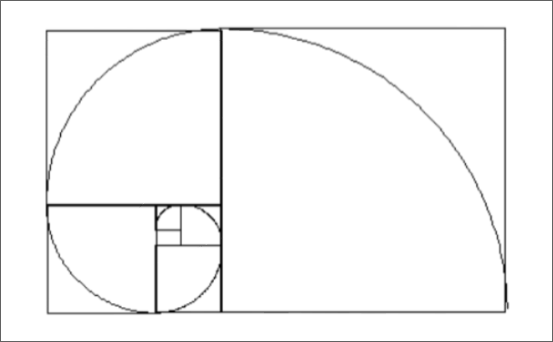
\includegraphics[width=0.8\textwidth]{images/golden_ratio.png}
    \caption{Golden ratio}
    \label{fig:Golden ratio}
  \end{minipage}
  \hfill
  \begin{minipage}{0.32\textwidth}
    \centering
    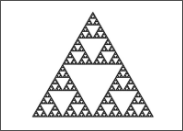
\includegraphics[width=0.6\textwidth]{images/sierpinski_triangle.jpeg}
    \caption{Sierpiński triangle}
    \label{fig:Sierpiński triangle}
  \end{minipage}
  \hfill
  \begin{minipage}{0.32\textwidth}
    \centering
    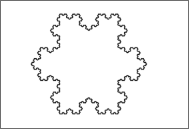
\includegraphics[width=0.6\textwidth]{images/koch_flake.png}
    \caption{Koch flake}
    \label{fig:Kochflake}
  \end{minipage}

\end{figure}

In order to be able to work with fractals nonetheless, we can use visualize by recursion with a relatively high recursion depth.
The depth of recursion is the scale of sharpness fractal images have.

\subsection{Koch flake}

The Koch flake became quite popular for its simplistic form and minimal lines of code for a quite nice looking shape of a snowflake.
First, described by Helge von Koch in 1904. It is made up of three triangular shaped Koch curves which follow simple rules \cite{mathworld2}.

At first, a Koch curve is simply a line with a predefined length. By increasing the depth, Koch curves will be placed on top of these lines forming a triangular shaped spike on top of the base line.
Depth=0 is a straight line and the higher the depth, the more triangles are placed on top of each other.

We will declare our Koch curve in the same way we did with the Pythagoras tree.

\begin{lstlisting}
  to curve :length :depth
    ...
  end
\end{lstlisting}

We will start by defining our termination condition (\textit{base case}) by drawing a straight line.

\begin{lstlisting}[title=Part 1/4:]
  if :depth = 0 [fd :length stop]
\end{lstlisting}

To achieve our Koch curve with triangular placement, it consists of four parts:

The first quarter features a straight stretch that spans one-third of the total length. The second and third quarters represent the rotation, with both sides of the triangle placed at a depth on top. To finalise the curve, we perform the same process as in step one, covering a third of the length.

\begin{lstlisting}
  curve :length / 3 :depth - 1
  lt 60
  curve :length / 3 :depth - 1
  rt 120
  curve :length / 3 :depth - 1
  lt 60
  curve :length / 3 :depth - 1
\end{lstlisting}

To get a snowflake-shaped Koch flake we simply need to expend the Koch curve by another small procedure \textit{flake}.
This flake repeats our \textit{curve} three times and rotates 60 degree between each curve, so we end up having the shape of a triangle (\Cref{fig:Koch flake}).

\begin{lstlisting}[title={Koch flake}]
  to curve :length :depth
    forward and stop
    if :depth = 0 [fd :length stop]
    curve :length / 3 :depth - 1
    lt 60
    curve :length / 3 :depth - 1
     rt 120
    curve :length / 3 :depth - 1
    lt 60
    curve :length / 3 :depth - 1
  end

  to flake :depth
    repeat 3 [ curve 200 :depth rt 120 ]
  end
\end{lstlisting}

\section{Lindenmayer-systems}
\label{sec:Lsystem}
The Lindenmayer-system or short the L-system was invented by Aristid Lindenmayer in 1968.
He was a Hungarian biologist who wanted to recreate plant growth as accurately as possible.

For this purpose he came up with this $(V, \omega, P)$.
V is the alphabet, which consists of non-terminal and terminal symbols. Non-terminal symbols are symbols that will be replaced eventually, whereas terminal symbols will not be replaced at all.
$\omega$ is a non-empty starting word of an L-system which will be used to form new words that will be part of the L-system. These words are created with production rules $P$ \cite{lsystem}.

\subsection{Rewriting Methods}
This paper will only discuss the deterministic and context-free L-system. We start with an example to get the basic concept of these systems.

When looking at $(\{a,\ b\},\ a,\ P)$ where the production rule P describes $a \rightarrow ab$ which means that each time a word contains the letter $a$, it is replaced in the next step for $ab$ and $b \rightarrow bb$ which means that every $b$ will be replaced for $bb$. We start with the letter $a$ because our starting word $\omega =a$ in our system $a$ is replaced by $ab$. Now we have two letters in our word and each of them will be replaced simultaneously. This is a big difference compared to normal context-free languages where only one symbol is replaced at a time. $ab$ becomes $abbb$ because $a$ becomes $ab$ and $b$ turns into $bb$. Next, $abbb$ turns into $abbbbbbb$ (\Cref{bsp_productionrules}).

We will discuss two ways of creating an L-system using turtle graphics. They are edge-rewriting and node-rewriting. In these rewriting systems the alphabet $V=\{+,-,F\}$. These characters form words that can be interpreted in the turtle graphics. $+$ means turning the head of the turtle to the right and $-$ means turning to the left, both with a predefined angle that does not change in one system. and $F$ stands for going forward.
The production rules in edge-rewriting replace the $F$, the edges for a new shape. The edges in node-rewriting do not get replaced, there are new symbols $A\notin V$ that have no interpretation in the turtle-graphic. Their only purpose is to be replaced \cite{lsystem}.

\begin{figure}
  \centering
  \begin{align*}
    a &\rightarrow ab \\
    ab &\rightarrow abbb \\
    abbb &\rightarrow abbbbbbb \\
  \end{align*}
  \caption{Example of words in a deterministic and context-free L-system.}
  \label{bsp_productionrules}
\end{figure}

\subsubsection{Edge-rewriting}
Edge-rewriting is the more intuitive way of creating L-systems. For example, \Cref{edge_bsp} shows an L-system $(\{+,-,F\},F,P)$ with $P:=F \rightarrow +F-F$ and an angle $\delta=45$°. As mentioned earlier, L-systems have terminal symbols and non-terminal symbols. In our example $\{+,-\}$ are terminal symbols, they do not get replaced by our production rules and $F$ is a non-terminal symbol since we have a rule for replacing $F$ with something else. However, our $F$ already had a meaning being an edge in our L-system. This edge in our example (\Cref{edge_bsp} image 1.) (depth=0) is replaced by a shape (\Cref{edge_bsp} image 2.) (depth=1).

There is also the possibility to use two $F$s, for example having now $F_r$ and $F_l$ for more variation and complexity in our L-system. In \Cref{edge_bsp} we see the difference between one rule in image 3.1 and two rules in image 3.2, both with depth=2. We define $P:= F_r\rightarrow +F_r-F_l ,\ F_l\rightarrow -F_r+F_l$ and the starting word $\omega=F_r$. The first rule is the same rule as in the earlier example and our second rule is the same shape to replace our lines but mirrored to the first rule. As seen in \Cref{edge_bsp} image 3.2, with two reproduction rules, the image looks more complex \cite{lsystem}.

\begin{figure}[h]
  \centering
  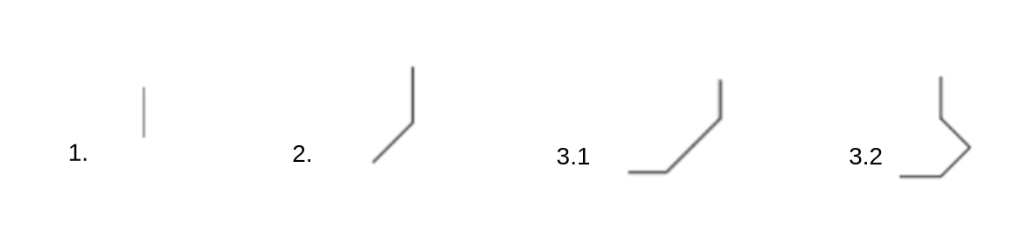
\includegraphics[width=0.5\linewidth]{images/edge_bsp.png}
  \caption{Example of L-system using edge-rewriting.}
  \label{edge_bsp}
\end{figure}

\subsubsection{Node-rewriting}
For Node-rewriting we do not replace our edges $F$ anymore. We introduce new symbols $\{A,B,C,...\}$ that do not have any meaning in our system so far. We will only use the symbol $A$ in our example (\Cref{node_bsp}).

Our new L-system $(\{+,-,F,A\},FA,P)$ with $P:=A\rightarrow+AF-AF$ and an angle $\delta=45$°. Since the non-terminal symbols do not have any meaning, they do not change the image that we get by illustrating our L-system, but they determine how the next step of the recursion will look like. As you can see in \Cref{node_bsp}, the edge in image 1 (depth=0) stays in image 2 (depth=1), the edges in image 2. also stay in image 3.1 (depth=2). Just like with edge-rewriting, we can create L-systems with multiple rules. We define $P:= A_r\rightarrow+A_r F -A_l F,\ A_l\rightarrow-A_rF+A_lF$ and $\omega=FA_r$. The first two recursion steps look similar to the L-system with only one rule however in our example they differ with depth=2 in \Cref{node_bsp} image 3.1 with one rule and image 3.2 with two rules.

\begin{figure}[t]
  \centering
  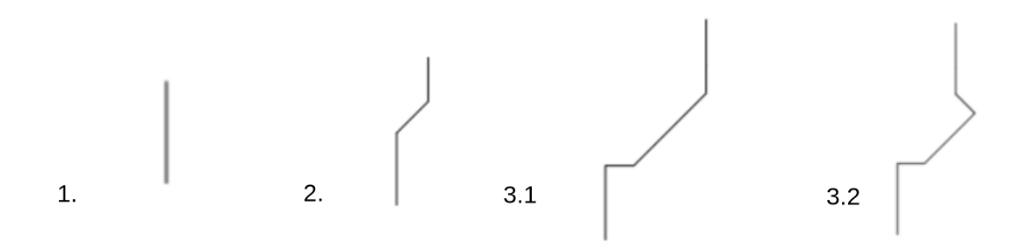
\includegraphics[width=0.5\linewidth]{images/node_bsp.png}
  \caption{Example of L-system using node-rewriting.}
  \label{node_bsp}
\end{figure}

\subsection{Designs}
Designs are essentially a repeated pattern of our fractal. To make our fractals look even more fabulous, the next step is to use designs. Designs are essentially a repeated pattern of our fractal. As we saw earlier with the Koch flake, this involves repeating the Koch curve three times. The first step is to choose a polygon on which to base the rewriting. In our example, we will choose a square. With our square, we now have four edges as a basis, whereas we only had one edge in our fractal. For edge rewriting, instead of replacing one line, we now have four lines, each of which is replaced by our shape. I. In  \cref{muster_bsp}, we can see that the two designs on the left were created using edge rewriting: the one on the left was created using one rule and the one on the right was created using two rules. We can do the same for node rewriting by placing nodes at the end of each edge, ensuring that every corner has a node. Each node is replaced by our rule for a shape. In our example, the two designs on the right in  \Cref{muster_bsp} were created using node rewriting. The design on the left was created using one rule and the design on the right was created using two rules. Whenever we replace edges or nodes in any polygon, the line always stops where it began (\Cref{muster_bsp}). All the designs in \Cref{muster_bsp} have depth=10.

\begin{figure}
  \centering
  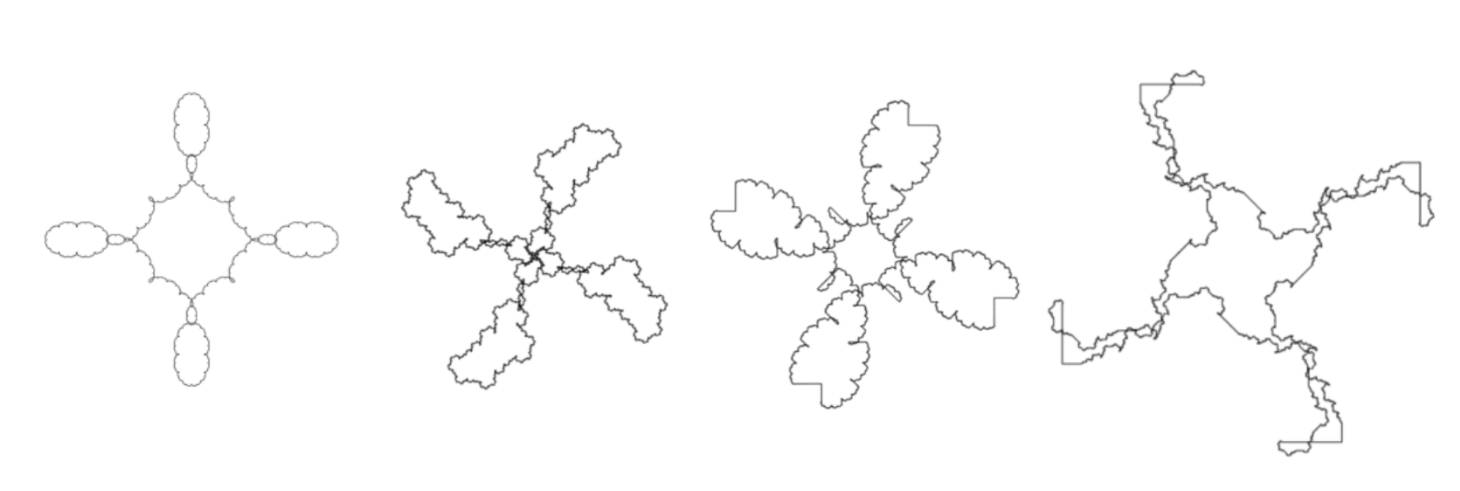
\includegraphics[width=0.5\linewidth]{images/muster_bsp.png}
  \caption{Designs created with our examples and a square.}
  \label{muster_bsp}
\end{figure}

\subsection{Branching}
Using edge-/node-rewriting, we can now create many L-systems. By using the turtle graphics, we can draw any number of angles and lines like the Pythagoras tree, the Koch flake or any self made L-system lines or designs. But they will always only be a line. However, the world of plants is nothing but a world of branching. Lindenmayer was a biologist and he wanted to recreate the world of plants. This can be achieved using either edge- or node-rewriting. We will only discuss it with edge-rewriting, but it works the same way for node-rewriting.

\subsubsection{Stack}
First, we need to know what a stack is and how it works for us to use branching.

A stack is a data structure that follows the principle of Last in First out or "LiFo". Two functions are used to operate the stack. The first function is \textit{push(input)}, when calling it, \textit{input} will be written in our stack. The second function is \textit{pop()}. It does not get any parameters and returns the last thing that was written on the stack removing it at the same time.

\subsubsection{Edge-rewriting with a Stack}
We will introduce two new symbols in our alphabet. We define $[:= push((position,direction))$ and $]:= pop()$. Every time we use $[$ in a word of our system, we save the current position and the direction the turtle is facing, and every time we read $]$ in our word the turtle returns to that position and the direction faced when we pushed that position. In our example we use the L-system $(\{-,+,F,[,]\},F,P)$ with $P:=F\rightarrow F[-F][+F]F$ and $\delta=45$°. We see that there are three branches, with depth=1 (\Cref{branch_bsp} image 2). In \Cref{branch_bsp} image 3 (depth=2) we can see why the stack is important and why we could not use a list or other data structures without "LiFo". The word for our 3. image is
$F[-F][+F]F[-F[-F][+F]F][+F[-F][+F]F]F[-F][+F]F$
and when we interleave the braces as we did in this example, we must ensure that the order of the returns is not mixed up, because if it were, our example would consist of three parts, which would mean that it would no longer be a fractal.

\begin{figure}[t]
  \centering
  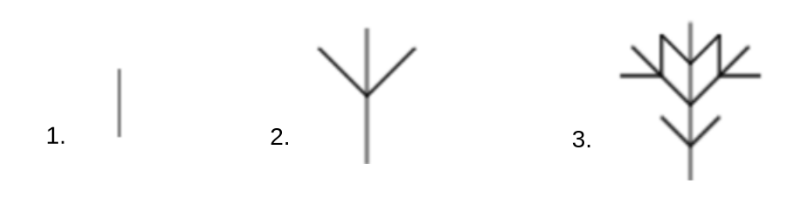
\includegraphics[width=0.5\linewidth]{images/branch_bsp.png}
  \caption{Example of branching with edge-rewriting.}
  \label{branch_bsp}
\end{figure}

\begin{figure}[h]
  \centering
  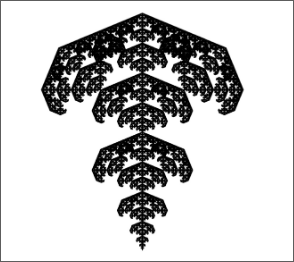
\includegraphics[width=0.3\linewidth]{images/flower.jpeg}
  \caption{Example of edge-rewriting with a stack}
  \label{flower}
\end{figure}

In \Cref{flower} we can see our example with depth=9. Now we have created a fractal that resembles a plant, and we can create many more, so we can now recreate a world of plants using branching.

\section{Conclusion}

We have learned some basic commands and data types, as well as how to create procedures in Logo. Furthermore, we now understand the key features that define recursion as a concept, and we have grasped the theoretical idea of fractals. Finally, we have learned how to create our own fractals. Edge-rewriting is more intuitive than node-rewriting, and using a stack enables us to create fractals that resemble plants.

\newpage
\printbibliography
\end{document}